% Content for Fourier Methods subsection
% This file is included in the main conference paper via % Content for Fourier Methods subsection
% This file is included in the main conference paper via % Content for Fourier Methods subsection
% This file is included in the main conference paper via % Content for Fourier Methods subsection
% This file is included in the main conference paper via \input{FourierMethods}

Two of the most prevalent transforms in signal processing are the Discrete Fourier Transform (DFT) and its derivative, the Discrete Cosine Transform (DCT). Broadly speaking, these transforms represent the original input as a sum of different wave frequencies. We will first discuss the DFT and its shortcomings, then show how this naturally gives rise to the DCT. 

\subsubsection{The Discrete Fourier Transform in 1 Dimension}

For the DFT, we consider our input as a 1-dimensional signal $x=\{x_0,\dots,x_{N-1}\}$ as described in Section \ref{methodsec:background}\footnote{We shift the indices to start at 0 throughout this section for convenience.}. For Fourier Analysis, it is common to call $x$ a \textbf{time signal}, which is any ordered list of values (in our case, the pixels along the rows and columns of the image). We assume that our signal is periodic modulo $N$, extending to infinity using the relation $x_k=x_{Nm+k}$ for each $m\in\mathbb{Z}$ as shown in Fig. \ref{fig:sigmod}. This way, we can define our basis to be the set of complex waveforms
\begin{equation}
    E=\{E_0,E_1,\dots,E_{N-1}\},\label{eq:dftbasis}
\end{equation}
where
\begin{equation}
    E_k=\{e^{2\pi ik(0)/N}, e^{2\pi ik(1)/N},\dots,e^{2\pi ik(N-1)/N}\}.\label{eq:dftbasiselement}
\end{equation}

\begin{figure}
    \centering
    \includestandalone[width=0.8\linewidth]{methods/Fourierdiagrams/SignalModN}
    \caption{The signal extension of $x\mod N$}
    \label{fig:sigmod}
\end{figure}

As a reminder, complex numbers are of the form $a+bi$, where $a,b\in\mathbb{R}$ and $i=\sqrt{-1}$. Also, we have Euler's identity
\begin{equation}
    e^{i\theta}=\cos\theta+i\sin\theta.
\end{equation}
This means that the basis is effectively made of discrete rotations around the unit circle in the complex plane at different frequencies. An example for the basis $E_1$ for $N=8$ is shown in Fig. \ref{fig:eulerid}. Note that the basis starts at 1 and travels around the unit circle clockwise.

\begin{figure}
    \centering
    \includestandalone[width=0.8\linewidth]{methods/Fourierdiagrams/EulersIdentity}
    \caption{The basis $E_1$ for $N=8$ in the complex plane. Note that these are all the solutions to $\omega^8=1$, the so-called 8th roots of unity.}
    \label{fig:eulerid}
\end{figure}

All of the basis vectors for $N=8$ are represented in Fig. \ref{fig:DFTBasis}, with both the real part (blue) and imaginary part (red). We have chosen $N=8$ for these figures as this will be our choice of block size for the 2D case later in this section. Note that the first basis vector $E_0$ is constant, while each subsequent vector has increasing frequency.

\begin{figure*}
    \centering
    \begin{minipage}{\textwidth}
        \centering
        \includestandalone[width=1\linewidth]{methods/Fourierdiagrams/DFTBasis}
    \end{minipage}
    \caption{Every DFT basis vector for $N=8$. The first row is $E_0,E_1,E_2,E_3$, and the second row is $E_4,E_5,E_6,E)7$. }
    \label{fig:DFTBasis}
\end{figure*}

We can transform the signal into a representation in our new basis using the following formula:
\begin{equation}
    X_k=\frac{1}{\sqrt{N}}\sum_{m=0}^{N-1}x_me^{-2\pi ikm/N}.\label{eq:dfttransform}
\end{equation}
This forms a new signal $X=\{X_0,X_2,\dots,X_{N-1}\}$ (note that the $1/\sqrt{N}$ term is just a normalization). We say that $X$ lives in the \textbf{frequency domain}. With the change of basis, each $X_k$ is now the corresponding coefficient for the basis vector $E_k$. The first coefficient $X_0$ is called the \textbf{DC coefficient}, and corresponds to the average value of the signal since $E_0$ is constant. All other coefficients are called \textbf{AC coefficients}\footnote{The terms DC and AC come from an electrical context, meaning \textit{direct current} and \textit{alternating current}}. This transform is lossless and invertible, with each value in the original time signal retrieved by calculating

\begin{equation}
    X_k=\frac{1}{\sqrt{N}}\sum_{m=0}^{N-1}X_me^{2\pi ikm/N}.\label{eq:idfttransform}
\end{equation}

We call equations \ref{eq:dfttransform} and \ref{eq:idfttransform} the \textbf{forward} and \textbf{inverse} transforms, respectively. These formulas are derived from taking the normal \textbf{inner product} in the vector space $\mathbb{C}^N$. Those interested in the mathematical background should refer to Broughton \cite{broughton2009discrete}. 

\subsubsection{Applying the Discrete Fourier Transform to a 2D Image}

We now discuss how to apply the 1D DFT to an image. As discussed in Section \ref{methodsec:background}, we represent the image as a 2D array of pixels in the YCbCr colorspace described in Section \ref{sec:intro}. We then break the image up into 8x8 blocks of pixels, and apply the 1D DFT along each row and each column of the block. A visualization for the transform is provided in Fig. \ref{fig:dftvis}.

\begin{figure}
    \centering
    
\includegraphics[width=0.4\linewidth]{methods/Fourierdiagrams/OriginalImg.png}\hfill
    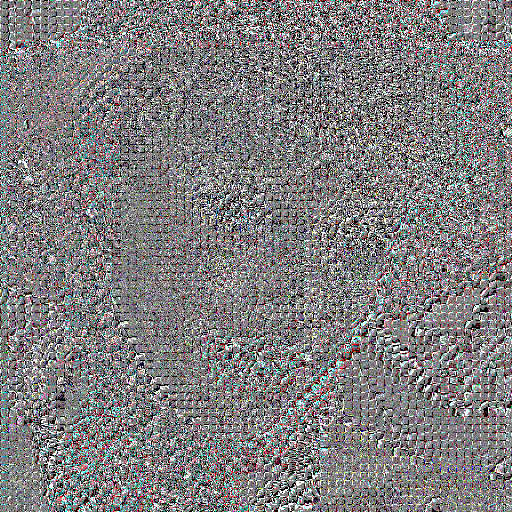
\includegraphics[width=0.4\linewidth]{methods/Fourierdiagrams/DFTVis.png}
    \caption{An original Image from the Kodak dataset (left) and a visualization after applying the DFT (right). The image is $512\times 512$ pixels, and at a closer look one can see block-like shapes where the transform has been applied to 8x8 chunks.}
    \label{fig:dftvis}
\end{figure}

In Section \ref{methodsec:background} we mentioned that the goal of the transform was to reduce entropy as defined in Section \ref{sec:intro}. If the image was random noise, we would generally not expect this to be the case. However, since pixels are correlated with those around them in an image, we don't expect sharp changes in pixel values. This means in our new basis, the coefficients for the lower frequency basis vectors $E_0,E_1,E_2,\dots$ have larger values than the coefficients for the higher frequency basis vectors $\dots,E_{N-2},E_{N-1}$. This results in a lower entropy, which combined with quantization discussed in Section \ref{methodsec:quant} allows for solid compression ratios.

\subsubsection{Problems with the DFT}
At this point, we have built up the DFT as a change of basis on an image to represent it as frequency components where we expect the energy of the signal to be concentrated in lower frequency coefficients. However, there are several problems that arise that greatly limit the ability of the DFT to achieve great compression.
\begin{enumerate}
    \item The DFT is slow. A raw application of Equation \ref{eq:dfttransform} requires $\mathcal{O}(N^2)$ complex multiplications, which means for a 2D Image the runtime is $\mathcal{O}(NM)^2$, for an $N\times M$ image (or just $\mathcal{O}(N^4)$ if we assume that the image is square).
    \item The output to the DFT is complex-valued. Since we are using complex waveforms as a basis, we are thinking of our pixels as living in the complex plane $\mathbb{C}$, not the real numbers $\mathbb{R}$. Complex values take twice as much space to store as real numbers.
    \item The DFT does not fully eliminate large values in high frequency coefficients. Since the DFT assumes the signal $x$ is periodic modulo $N$, if $|x_0-x_{N-1}|$ is large, then there will be a high frequency jump in the signal resulting in larger terms (Refer back to Fig. \ref{fig:sigmod} for an example). 
\end{enumerate}
The first issue of runtime can be addressed by using a clever algorithm called the Fast Fourier Transform (FFT), which exploits the symmetries of complex waveforms to reduce the runtime to $\mathcal{O}(N^2\log N)$ for an $N\times N$ pixel image. More details are provided in Appendix \ref{apx:fft}. At first glance, the following issues are not so easy to fix. However, by changing the assumptions about our signal $x$ slightly, we are able to solve both problems simultaneously. This is exactly what the Discrete Cosine Transform (DCT) does.

\subsubsection{The Discrete Cosine Transform}
The idea behind the DCT is very simple. Starting with our signal $x=\{x_0,\dots,x_{N-1}\}$, we first \textbf{mirror} our signal to one of length $2N$, giving a new signal
\begin{equation}
    \hat{x}=\{x_0,\dots,x_{N-1},x_{N-1},\dots,x_0\},
    \label{eq:dctsig}
\end{equation}
which we then assume is periodic modulo $2N$ instead as shown in Fig. \ref{fig:dctextension} in the $N=8$ case. We then perform the DFT on this extended signal to get a transformed signal $\hat{X}=\{X_0,\dots,X_{2N-1}\}$. With a little bit of unpacking, one can start with Equation \ref{eq:dfttransform} and show that the coefficients for the resulting transform are given by
\begin{align}
    X_k&=\sum_{m=0}^{2N-1}x_me^{-2\pi ikm/2N}\label{eq:2ndft}\\
    &=2e^{2\pi ik/2N}\sum_{m=0}^{N-1}x_m\cos\bigg(\frac{\pi k(m+\tfrac{1}{2})}{2N}\bigg),\label{eq:predcttransform}
\end{align}
where we have taken advantage of the symmetry in our mirrored signal $\hat{x}$. These terms are almost real, and after applying a phase shift and normalizing we get the final DCT coefficients given by
\begin{equation}
    X_k=\sqrt{\frac{c_k}{N}}\sum_{m=0}^{N-1}x_m\cos\bigg(\frac{\pi k(m+\tfrac{1}{2})}{N}\bigg),\label{eq:dcttransform}
\end{equation}
taking $c_k=1$ if $k=0$ and $c_k=2$ otherwise. Note that this gives us only half of the $2N$ coefficients that we expect. This is sufficient because due to the symmetry of the signal, the remaining coefficients are recovered by the identity
\begin{equation}
    X_{2N-r}=-X_r\quad\text{for }r=0,1,\dots,N.\label{eq:dctrelation}
\end{equation}
Notice that this forces $X_N=0$. The math behind these relations can be found in Broughton \cite{broughton2009discrete}. We now notice the 2 critical facts about the result.
\begin{enumerate}
    \item The DCT is real-valued. The mirrored nature of the extended signal $\hat{x}$ has washed out all imaginary components.
    \item The new signal also has no potential for sharp gaps when moving to a new period, meaning smaller values in the higher frequency coefficients.
\end{enumerate}
These are exactly the two problems that we wanted to improve on for the DFT, and we see that the DCT achieves both by mirroring the signal and using the relation in Equation \ref{eq:dctrelation} to not increase space. To apply the DCT to an image, one can simply follow the same steps for the DFT, except to mirror each row and each column of pixels in each chunk before applying the transform, and saving the first half of the result. See Section \ref{sec:results} for just how much more effective the DCT is over the DFT.

\begin{figure}
    \centering
    \includestandalone[width=0.8\linewidth]{methods/Fourierdiagrams/DCTExtension}
    \caption{The new signal $\hat{x}$ extended modulo $2N$ for $N=8$. Note that there are no sharp gaps at the extension point.}
    \label{fig:dctextension}
\end{figure}

Two of the most prevalent transforms in signal processing are the Discrete Fourier Transform (DFT) and its derivative, the Discrete Cosine Transform (DCT). Broadly speaking, these transforms represent the original input as a sum of different wave frequencies. We will first discuss the DFT and its shortcomings, then show how this naturally gives rise to the DCT. 

\subsubsection{The Discrete Fourier Transform in 1 Dimension}

For the DFT, we consider our input as a 1-dimensional signal $x=\{x_0,\dots,x_{N-1}\}$ as described in Section \ref{methodsec:background}\footnote{We shift the indices to start at 0 throughout this section for convenience.}. For Fourier Analysis, it is common to call $x$ a \textbf{time signal}, which is any ordered list of values (in our case, the pixels along the rows and columns of the image). We assume that our signal is periodic modulo $N$, extending to infinity using the relation $x_k=x_{Nm+k}$ for each $m\in\mathbb{Z}$ as shown in Fig. \ref{fig:sigmod}. This way, we can define our basis to be the set of complex waveforms
\begin{equation}
    E=\{E_0,E_1,\dots,E_{N-1}\},\label{eq:dftbasis}
\end{equation}
where
\begin{equation}
    E_k=\{e^{2\pi ik(0)/N}, e^{2\pi ik(1)/N},\dots,e^{2\pi ik(N-1)/N}\}.\label{eq:dftbasiselement}
\end{equation}

\begin{figure}
    \centering
    \includestandalone[width=0.8\linewidth]{methods/Fourierdiagrams/SignalModN}
    \caption{The signal extension of $x\mod N$}
    \label{fig:sigmod}
\end{figure}

As a reminder, complex numbers are of the form $a+bi$, where $a,b\in\mathbb{R}$ and $i=\sqrt{-1}$. Also, we have Euler's identity
\begin{equation}
    e^{i\theta}=\cos\theta+i\sin\theta.
\end{equation}
This means that the basis is effectively made of discrete rotations around the unit circle in the complex plane at different frequencies. An example for the basis $E_1$ for $N=8$ is shown in Fig. \ref{fig:eulerid}. Note that the basis starts at 1 and travels around the unit circle clockwise.

\begin{figure}
    \centering
    \includestandalone[width=0.8\linewidth]{methods/Fourierdiagrams/EulersIdentity}
    \caption{The basis $E_1$ for $N=8$ in the complex plane. Note that these are all the solutions to $\omega^8=1$, the so-called 8th roots of unity.}
    \label{fig:eulerid}
\end{figure}

All of the basis vectors for $N=8$ are represented in Fig. \ref{fig:DFTBasis}, with both the real part (blue) and imaginary part (red). We have chosen $N=8$ for these figures as this will be our choice of block size for the 2D case later in this section. Note that the first basis vector $E_0$ is constant, while each subsequent vector has increasing frequency.

\begin{figure*}
    \centering
    \begin{minipage}{\textwidth}
        \centering
        \includestandalone[width=1\linewidth]{methods/Fourierdiagrams/DFTBasis}
    \end{minipage}
    \caption{Every DFT basis vector for $N=8$. The first row is $E_0,E_1,E_2,E_3$, and the second row is $E_4,E_5,E_6,E)7$. }
    \label{fig:DFTBasis}
\end{figure*}

We can transform the signal into a representation in our new basis using the following formula:
\begin{equation}
    X_k=\frac{1}{\sqrt{N}}\sum_{m=0}^{N-1}x_me^{-2\pi ikm/N}.\label{eq:dfttransform}
\end{equation}
This forms a new signal $X=\{X_0,X_2,\dots,X_{N-1}\}$ (note that the $1/\sqrt{N}$ term is just a normalization). We say that $X$ lives in the \textbf{frequency domain}. With the change of basis, each $X_k$ is now the corresponding coefficient for the basis vector $E_k$. The first coefficient $X_0$ is called the \textbf{DC coefficient}, and corresponds to the average value of the signal since $E_0$ is constant. All other coefficients are called \textbf{AC coefficients}\footnote{The terms DC and AC come from an electrical context, meaning \textit{direct current} and \textit{alternating current}}. This transform is lossless and invertible, with each value in the original time signal retrieved by calculating

\begin{equation}
    X_k=\frac{1}{\sqrt{N}}\sum_{m=0}^{N-1}X_me^{2\pi ikm/N}.\label{eq:idfttransform}
\end{equation}

We call equations \ref{eq:dfttransform} and \ref{eq:idfttransform} the \textbf{forward} and \textbf{inverse} transforms, respectively. These formulas are derived from taking the normal \textbf{inner product} in the vector space $\mathbb{C}^N$. Those interested in the mathematical background should refer to Broughton \cite{broughton2009discrete}. 

\subsubsection{Applying the Discrete Fourier Transform to a 2D Image}

We now discuss how to apply the 1D DFT to an image. As discussed in Section \ref{methodsec:background}, we represent the image as a 2D array of pixels in the YCbCr colorspace described in Section \ref{sec:intro}. We then break the image up into 8x8 blocks of pixels, and apply the 1D DFT along each row and each column of the block. A visualization for the transform is provided in Fig. \ref{fig:dftvis}.

\begin{figure}
    \centering
    
\includegraphics[width=0.4\linewidth]{methods/Fourierdiagrams/OriginalImg.png}\hfill
    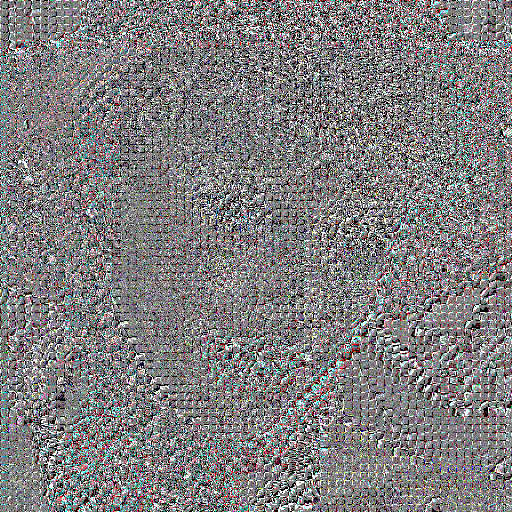
\includegraphics[width=0.4\linewidth]{methods/Fourierdiagrams/DFTVis.png}
    \caption{An original Image from the Kodak dataset (left) and a visualization after applying the DFT (right). The image is $512\times 512$ pixels, and at a closer look one can see block-like shapes where the transform has been applied to 8x8 chunks.}
    \label{fig:dftvis}
\end{figure}

In Section \ref{methodsec:background} we mentioned that the goal of the transform was to reduce entropy as defined in Section \ref{sec:intro}. If the image was random noise, we would generally not expect this to be the case. However, since pixels are correlated with those around them in an image, we don't expect sharp changes in pixel values. This means in our new basis, the coefficients for the lower frequency basis vectors $E_0,E_1,E_2,\dots$ have larger values than the coefficients for the higher frequency basis vectors $\dots,E_{N-2},E_{N-1}$. This results in a lower entropy, which combined with quantization discussed in Section \ref{methodsec:quant} allows for solid compression ratios.

\subsubsection{Problems with the DFT}
At this point, we have built up the DFT as a change of basis on an image to represent it as frequency components where we expect the energy of the signal to be concentrated in lower frequency coefficients. However, there are several problems that arise that greatly limit the ability of the DFT to achieve great compression.
\begin{enumerate}
    \item The DFT is slow. A raw application of Equation \ref{eq:dfttransform} requires $\mathcal{O}(N^2)$ complex multiplications, which means for a 2D Image the runtime is $\mathcal{O}(NM)^2$, for an $N\times M$ image (or just $\mathcal{O}(N^4)$ if we assume that the image is square).
    \item The output to the DFT is complex-valued. Since we are using complex waveforms as a basis, we are thinking of our pixels as living in the complex plane $\mathbb{C}$, not the real numbers $\mathbb{R}$. Complex values take twice as much space to store as real numbers.
    \item The DFT does not fully eliminate large values in high frequency coefficients. Since the DFT assumes the signal $x$ is periodic modulo $N$, if $|x_0-x_{N-1}|$ is large, then there will be a high frequency jump in the signal resulting in larger terms (Refer back to Fig. \ref{fig:sigmod} for an example). 
\end{enumerate}
The first issue of runtime can be addressed by using a clever algorithm called the Fast Fourier Transform (FFT), which exploits the symmetries of complex waveforms to reduce the runtime to $\mathcal{O}(N^2\log N)$ for an $N\times N$ pixel image. More details are provided in Appendix \ref{apx:fft}. At first glance, the following issues are not so easy to fix. However, by changing the assumptions about our signal $x$ slightly, we are able to solve both problems simultaneously. This is exactly what the Discrete Cosine Transform (DCT) does.

\subsubsection{The Discrete Cosine Transform}
The idea behind the DCT is very simple. Starting with our signal $x=\{x_0,\dots,x_{N-1}\}$, we first \textbf{mirror} our signal to one of length $2N$, giving a new signal
\begin{equation}
    \hat{x}=\{x_0,\dots,x_{N-1},x_{N-1},\dots,x_0\},
    \label{eq:dctsig}
\end{equation}
which we then assume is periodic modulo $2N$ instead as shown in Fig. \ref{fig:dctextension} in the $N=8$ case. We then perform the DFT on this extended signal to get a transformed signal $\hat{X}=\{X_0,\dots,X_{2N-1}\}$. With a little bit of unpacking, one can start with Equation \ref{eq:dfttransform} and show that the coefficients for the resulting transform are given by
\begin{align}
    X_k&=\sum_{m=0}^{2N-1}x_me^{-2\pi ikm/2N}\label{eq:2ndft}\\
    &=2e^{2\pi ik/2N}\sum_{m=0}^{N-1}x_m\cos\bigg(\frac{\pi k(m+\tfrac{1}{2})}{2N}\bigg),\label{eq:predcttransform}
\end{align}
where we have taken advantage of the symmetry in our mirrored signal $\hat{x}$. These terms are almost real, and after applying a phase shift and normalizing we get the final DCT coefficients given by
\begin{equation}
    X_k=\sqrt{\frac{c_k}{N}}\sum_{m=0}^{N-1}x_m\cos\bigg(\frac{\pi k(m+\tfrac{1}{2})}{N}\bigg),\label{eq:dcttransform}
\end{equation}
taking $c_k=1$ if $k=0$ and $c_k=2$ otherwise. Note that this gives us only half of the $2N$ coefficients that we expect. This is sufficient because due to the symmetry of the signal, the remaining coefficients are recovered by the identity
\begin{equation}
    X_{2N-r}=-X_r\quad\text{for }r=0,1,\dots,N.\label{eq:dctrelation}
\end{equation}
Notice that this forces $X_N=0$. The math behind these relations can be found in Broughton \cite{broughton2009discrete}. We now notice the 2 critical facts about the result.
\begin{enumerate}
    \item The DCT is real-valued. The mirrored nature of the extended signal $\hat{x}$ has washed out all imaginary components.
    \item The new signal also has no potential for sharp gaps when moving to a new period, meaning smaller values in the higher frequency coefficients.
\end{enumerate}
These are exactly the two problems that we wanted to improve on for the DFT, and we see that the DCT achieves both by mirroring the signal and using the relation in Equation \ref{eq:dctrelation} to not increase space. To apply the DCT to an image, one can simply follow the same steps for the DFT, except to mirror each row and each column of pixels in each chunk before applying the transform, and saving the first half of the result. See Section \ref{sec:results} for just how much more effective the DCT is over the DFT.

\begin{figure}
    \centering
    \includestandalone[width=0.8\linewidth]{methods/Fourierdiagrams/DCTExtension}
    \caption{The new signal $\hat{x}$ extended modulo $2N$ for $N=8$. Note that there are no sharp gaps at the extension point.}
    \label{fig:dctextension}
\end{figure}

Two of the most prevalent transforms in signal processing are the Discrete Fourier Transform (DFT) and its derivative, the Discrete Cosine Transform (DCT). Broadly speaking, these transforms represent the original input as a sum of different wave frequencies. We will first discuss the DFT and its shortcomings, then show how this naturally gives rise to the DCT. 

\subsubsection{The Discrete Fourier Transform in 1 Dimension}

For the DFT, we consider our input as a 1-dimensional signal $x=\{x_0,\dots,x_{N-1}\}$ as described in Section \ref{methodsec:background}\footnote{We shift the indices to start at 0 throughout this section for convenience.}. For Fourier Analysis, it is common to call $x$ a \textbf{time signal}, which is any ordered list of values (in our case, the pixels along the rows and columns of the image). We assume that our signal is periodic modulo $N$, extending to infinity using the relation $x_k=x_{Nm+k}$ for each $m\in\mathbb{Z}$ as shown in Fig. \ref{fig:sigmod}. This way, we can define our basis to be the set of complex waveforms
\begin{equation}
    E=\{E_0,E_1,\dots,E_{N-1}\},\label{eq:dftbasis}
\end{equation}
where
\begin{equation}
    E_k=\{e^{2\pi ik(0)/N}, e^{2\pi ik(1)/N},\dots,e^{2\pi ik(N-1)/N}\}.\label{eq:dftbasiselement}
\end{equation}

\begin{figure}
    \centering
    \includestandalone[width=0.8\linewidth]{methods/Fourierdiagrams/SignalModN}
    \caption{The signal extension of $x\mod N$}
    \label{fig:sigmod}
\end{figure}

As a reminder, complex numbers are of the form $a+bi$, where $a,b\in\mathbb{R}$ and $i=\sqrt{-1}$. Also, we have Euler's identity
\begin{equation}
    e^{i\theta}=\cos\theta+i\sin\theta.
\end{equation}
This means that the basis is effectively made of discrete rotations around the unit circle in the complex plane at different frequencies. An example for the basis $E_1$ for $N=8$ is shown in Fig. \ref{fig:eulerid}. Note that the basis starts at 1 and travels around the unit circle clockwise.

\begin{figure}
    \centering
    \includestandalone[width=0.8\linewidth]{methods/Fourierdiagrams/EulersIdentity}
    \caption{The basis $E_1$ for $N=8$ in the complex plane. Note that these are all the solutions to $\omega^8=1$, the so-called 8th roots of unity.}
    \label{fig:eulerid}
\end{figure}

All of the basis vectors for $N=8$ are represented in Fig. \ref{fig:DFTBasis}, with both the real part (blue) and imaginary part (red). We have chosen $N=8$ for these figures as this will be our choice of block size for the 2D case later in this section. Note that the first basis vector $E_0$ is constant, while each subsequent vector has increasing frequency.

\begin{figure*}
    \centering
    \begin{minipage}{\textwidth}
        \centering
        \includestandalone[width=1\linewidth]{methods/Fourierdiagrams/DFTBasis}
    \end{minipage}
    \caption{Every DFT basis vector for $N=8$. The first row is $E_0,E_1,E_2,E_3$, and the second row is $E_4,E_5,E_6,E)7$. }
    \label{fig:DFTBasis}
\end{figure*}

We can transform the signal into a representation in our new basis using the following formula:
\begin{equation}
    X_k=\frac{1}{\sqrt{N}}\sum_{m=0}^{N-1}x_me^{-2\pi ikm/N}.\label{eq:dfttransform}
\end{equation}
This forms a new signal $X=\{X_0,X_2,\dots,X_{N-1}\}$ (note that the $1/\sqrt{N}$ term is just a normalization). We say that $X$ lives in the \textbf{frequency domain}. With the change of basis, each $X_k$ is now the corresponding coefficient for the basis vector $E_k$. The first coefficient $X_0$ is called the \textbf{DC coefficient}, and corresponds to the average value of the signal since $E_0$ is constant. All other coefficients are called \textbf{AC coefficients}\footnote{The terms DC and AC come from an electrical context, meaning \textit{direct current} and \textit{alternating current}}. This transform is lossless and invertible, with each value in the original time signal retrieved by calculating

\begin{equation}
    X_k=\frac{1}{\sqrt{N}}\sum_{m=0}^{N-1}X_me^{2\pi ikm/N}.\label{eq:idfttransform}
\end{equation}

We call equations \ref{eq:dfttransform} and \ref{eq:idfttransform} the \textbf{forward} and \textbf{inverse} transforms, respectively. These formulas are derived from taking the normal \textbf{inner product} in the vector space $\mathbb{C}^N$. Those interested in the mathematical background should refer to Broughton \cite{broughton2009discrete}. 

\subsubsection{Applying the Discrete Fourier Transform to a 2D Image}

We now discuss how to apply the 1D DFT to an image. As discussed in Section \ref{methodsec:background}, we represent the image as a 2D array of pixels in the YCbCr colorspace described in Section \ref{sec:intro}. We then break the image up into 8x8 blocks of pixels, and apply the 1D DFT along each row and each column of the block. A visualization for the transform is provided in Fig. \ref{fig:dftvis}.

\begin{figure}
    \centering
    
\includegraphics[width=0.4\linewidth]{methods/Fourierdiagrams/OriginalImg.png}\hfill
    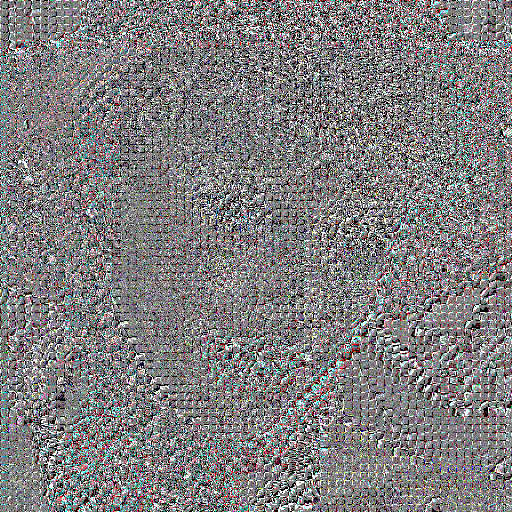
\includegraphics[width=0.4\linewidth]{methods/Fourierdiagrams/DFTVis.png}
    \caption{An original Image from the Kodak dataset (left) and a visualization after applying the DFT (right). The image is $512\times 512$ pixels, and at a closer look one can see block-like shapes where the transform has been applied to 8x8 chunks.}
    \label{fig:dftvis}
\end{figure}

In Section \ref{methodsec:background} we mentioned that the goal of the transform was to reduce entropy as defined in Section \ref{sec:intro}. If the image was random noise, we would generally not expect this to be the case. However, since pixels are correlated with those around them in an image, we don't expect sharp changes in pixel values. This means in our new basis, the coefficients for the lower frequency basis vectors $E_0,E_1,E_2,\dots$ have larger values than the coefficients for the higher frequency basis vectors $\dots,E_{N-2},E_{N-1}$. This results in a lower entropy, which combined with quantization discussed in Section \ref{methodsec:quant} allows for solid compression ratios.

\subsubsection{Problems with the DFT}
At this point, we have built up the DFT as a change of basis on an image to represent it as frequency components where we expect the energy of the signal to be concentrated in lower frequency coefficients. However, there are several problems that arise that greatly limit the ability of the DFT to achieve great compression.
\begin{enumerate}
    \item The DFT is slow. A raw application of Equation \ref{eq:dfttransform} requires $\mathcal{O}(N^2)$ complex multiplications, which means for a 2D Image the runtime is $\mathcal{O}(NM)^2$, for an $N\times M$ image (or just $\mathcal{O}(N^4)$ if we assume that the image is square).
    \item The output to the DFT is complex-valued. Since we are using complex waveforms as a basis, we are thinking of our pixels as living in the complex plane $\mathbb{C}$, not the real numbers $\mathbb{R}$. Complex values take twice as much space to store as real numbers.
    \item The DFT does not fully eliminate large values in high frequency coefficients. Since the DFT assumes the signal $x$ is periodic modulo $N$, if $|x_0-x_{N-1}|$ is large, then there will be a high frequency jump in the signal resulting in larger terms (Refer back to Fig. \ref{fig:sigmod} for an example). 
\end{enumerate}
The first issue of runtime can be addressed by using a clever algorithm called the Fast Fourier Transform (FFT), which exploits the symmetries of complex waveforms to reduce the runtime to $\mathcal{O}(N^2\log N)$ for an $N\times N$ pixel image. More details are provided in Appendix \ref{apx:fft}. At first glance, the following issues are not so easy to fix. However, by changing the assumptions about our signal $x$ slightly, we are able to solve both problems simultaneously. This is exactly what the Discrete Cosine Transform (DCT) does.

\subsubsection{The Discrete Cosine Transform}
The idea behind the DCT is very simple. Starting with our signal $x=\{x_0,\dots,x_{N-1}\}$, we first \textbf{mirror} our signal to one of length $2N$, giving a new signal
\begin{equation}
    \hat{x}=\{x_0,\dots,x_{N-1},x_{N-1},\dots,x_0\},
    \label{eq:dctsig}
\end{equation}
which we then assume is periodic modulo $2N$ instead as shown in Fig. \ref{fig:dctextension} in the $N=8$ case. We then perform the DFT on this extended signal to get a transformed signal $\hat{X}=\{X_0,\dots,X_{2N-1}\}$. With a little bit of unpacking, one can start with Equation \ref{eq:dfttransform} and show that the coefficients for the resulting transform are given by
\begin{align}
    X_k&=\sum_{m=0}^{2N-1}x_me^{-2\pi ikm/2N}\label{eq:2ndft}\\
    &=2e^{2\pi ik/2N}\sum_{m=0}^{N-1}x_m\cos\bigg(\frac{\pi k(m+\tfrac{1}{2})}{2N}\bigg),\label{eq:predcttransform}
\end{align}
where we have taken advantage of the symmetry in our mirrored signal $\hat{x}$. These terms are almost real, and after applying a phase shift and normalizing we get the final DCT coefficients given by
\begin{equation}
    X_k=\sqrt{\frac{c_k}{N}}\sum_{m=0}^{N-1}x_m\cos\bigg(\frac{\pi k(m+\tfrac{1}{2})}{N}\bigg),\label{eq:dcttransform}
\end{equation}
taking $c_k=1$ if $k=0$ and $c_k=2$ otherwise. Note that this gives us only half of the $2N$ coefficients that we expect. This is sufficient because due to the symmetry of the signal, the remaining coefficients are recovered by the identity
\begin{equation}
    X_{2N-r}=-X_r\quad\text{for }r=0,1,\dots,N.\label{eq:dctrelation}
\end{equation}
Notice that this forces $X_N=0$. The math behind these relations can be found in Broughton \cite{broughton2009discrete}. We now notice the 2 critical facts about the result.
\begin{enumerate}
    \item The DCT is real-valued. The mirrored nature of the extended signal $\hat{x}$ has washed out all imaginary components.
    \item The new signal also has no potential for sharp gaps when moving to a new period, meaning smaller values in the higher frequency coefficients.
\end{enumerate}
These are exactly the two problems that we wanted to improve on for the DFT, and we see that the DCT achieves both by mirroring the signal and using the relation in Equation \ref{eq:dctrelation} to not increase space. To apply the DCT to an image, one can simply follow the same steps for the DFT, except to mirror each row and each column of pixels in each chunk before applying the transform, and saving the first half of the result. See Section \ref{sec:results} for just how much more effective the DCT is over the DFT.

\begin{figure}
    \centering
    \includestandalone[width=0.8\linewidth]{methods/Fourierdiagrams/DCTExtension}
    \caption{The new signal $\hat{x}$ extended modulo $2N$ for $N=8$. Note that there are no sharp gaps at the extension point.}
    \label{fig:dctextension}
\end{figure}

Two of the most prevalent transforms in signal processing are the Discrete Fourier Transform (DFT) and its derivative, the Discrete Cosine Transform (DCT). Broadly speaking, these transforms represent the original input as a sum of different wave frequencies. We will first discuss the DFT and its shortcomings, then show how this naturally gives rise to the DCT. 

\subsubsection{The Discrete Fourier Transform in 1 Dimension}

For the DFT, we consider our input as a 1-dimensional signal $x=\{x_0,\dots,x_{N-1}\}$ as described in Section \ref{methodsec:background}\footnote{We shift the indices to start at 0 throughout this section for convenience.}. For Fourier Analysis, it is common to call $x$ a \textbf{time signal}, which is any ordered list of values (in our case, the pixels along the rows and columns of the image). We assume that our signal is periodic modulo $N$, extending to infinity using the relation $x_k=x_{Nm+k}$ for each $m\in\mathbb{Z}$ as shown in Fig. \ref{fig:sigmod}. This way, we can define our basis to be the set of complex waveforms
\begin{equation}
    E=\{E_0,E_1,\dots,E_{N-1}\},\label{eq:dftbasis}
\end{equation}
where
\begin{equation}
    E_k=\{e^{2\pi ik(0)/N}, e^{2\pi ik(1)/N},\dots,e^{2\pi ik(N-1)/N}\}.\label{eq:dftbasiselement}
\end{equation}

\begin{figure}
    \centering
    \includestandalone[width=0.8\linewidth]{methods/Fourierdiagrams/SignalModN}
    \caption{The signal extension of $x\mod N$}
    \label{fig:sigmod}
\end{figure}

As a reminder, complex numbers are of the form $a+bi$, where $a,b\in\mathbb{R}$ and $i=\sqrt{-1}$. Also, we have Euler's identity
\begin{equation}
    e^{i\theta}=\cos\theta+i\sin\theta.
\end{equation}
This means that the basis is effectively made of discrete rotations around the unit circle in the complex plane at different frequencies. An example for the basis $E_1$ for $N=8$ is shown in Fig. \ref{fig:eulerid}. Note that the basis starts at 1 and travels around the unit circle clockwise.

\begin{figure}
    \centering
    \includestandalone[width=0.8\linewidth]{methods/Fourierdiagrams/EulersIdentity}
    \caption{The basis $E_1$ for $N=8$ in the complex plane. Note that these are all the solutions to $\omega^8=1$, the so-called 8th roots of unity.}
    \label{fig:eulerid}
\end{figure}

All of the basis vectors for $N=8$ are represented in Fig. \ref{fig:DFTBasis}, with both the real part (blue) and imaginary part (red). We have chosen $N=8$ for these figures as this will be our choice of block size for the 2D case later in this section. Note that the first basis vector $E_0$ is constant, while each subsequent vector has increasing frequency.

\begin{figure*}
    \centering
    \begin{minipage}{\textwidth}
        \centering
        \includestandalone[width=1\linewidth]{methods/Fourierdiagrams/DFTBasis}
    \end{minipage}
    \caption{Every DFT basis vector for $N=8$. The first row is $E_0,E_1,E_2,E_3$, and the second row is $E_4,E_5,E_6,E)7$. }
    \label{fig:DFTBasis}
\end{figure*}

We can transform the signal into a representation in our new basis using the following formula:
\begin{equation}
    X_k=\frac{1}{\sqrt{N}}\sum_{m=0}^{N-1}x_me^{-2\pi ikm/N}.\label{eq:dfttransform}
\end{equation}
This forms a new signal $X=\{X_0,X_2,\dots,X_{N-1}\}$ (note that the $1/\sqrt{N}$ term is just a normalization). We say that $X$ lives in the \textbf{frequency domain}. With the change of basis, each $X_k$ is now the corresponding coefficient for the basis vector $E_k$. The first coefficient $X_0$ is called the \textbf{DC coefficient}, and corresponds to the average value of the signal since $E_0$ is constant. All other coefficients are called \textbf{AC coefficients}\footnote{The terms DC and AC come from an electrical context, meaning \textit{direct current} and \textit{alternating current}}. This transform is lossless and invertible, with each value in the original time signal retrieved by calculating

\begin{equation}
    X_k=\frac{1}{\sqrt{N}}\sum_{m=0}^{N-1}X_me^{2\pi ikm/N}.\label{eq:idfttransform}
\end{equation}

We call equations \ref{eq:dfttransform} and \ref{eq:idfttransform} the \textbf{forward} and \textbf{inverse} transforms, respectively. These formulas are derived from taking the normal \textbf{inner product} in the vector space $\mathbb{C}^N$. Those interested in the mathematical background should refer to Broughton \cite{broughton2009discrete}. 

\subsubsection{Applying the Discrete Fourier Transform to a 2D Image}

We now discuss how to apply the 1D DFT to an image. As discussed in Section \ref{methodsec:background}, we represent the image as a 2D array of pixels in the YCbCr colorspace described in Section \ref{sec:intro}. We then break the image up into 8x8 blocks of pixels, and apply the 1D DFT along each row and each column of the block. A visualization for the transform is provided in Fig. \ref{fig:dftvis}.

\begin{figure}
    \centering
    
\includegraphics[width=0.4\linewidth]{methods/Fourierdiagrams/OriginalImg.png}\hfill
    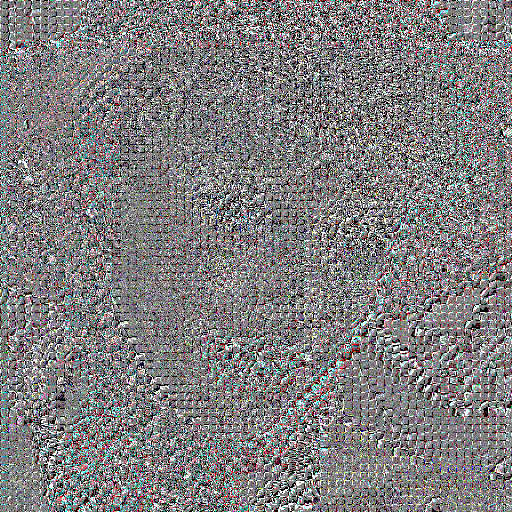
\includegraphics[width=0.4\linewidth]{methods/Fourierdiagrams/DFTVis.png}
    \caption{An original Image from the Kodak dataset (left) and a visualization after applying the DFT (right). The image is $512\times 512$ pixels, and at a closer look one can see block-like shapes where the transform has been applied to 8x8 chunks.}
    \label{fig:dftvis}
\end{figure}

In Section \ref{methodsec:background} we mentioned that the goal of the transform was to reduce entropy as defined in Section \ref{sec:intro}. If the image was random noise, we would generally not expect this to be the case. However, since pixels are correlated with those around them in an image, we don't expect sharp changes in pixel values. This means in our new basis, the coefficients for the lower frequency basis vectors $E_0,E_1,E_2,\dots$ have larger values than the coefficients for the higher frequency basis vectors $\dots,E_{N-2},E_{N-1}$. This results in a lower entropy, which combined with quantization discussed in Section \ref{methodsec:quant} allows for solid compression ratios.

\subsubsection{Problems with the DFT}
At this point, we have built up the DFT as a change of basis on an image to represent it as frequency components where we expect the energy of the signal to be concentrated in lower frequency coefficients. However, there are several problems that arise that greatly limit the ability of the DFT to achieve great compression.
\begin{enumerate}
    \item The DFT is slow. A raw application of Equation \ref{eq:dfttransform} requires $\mathcal{O}(N^2)$ complex multiplications, which means for a 2D Image the runtime is $\mathcal{O}(NM)^2$, for an $N\times M$ image (or just $\mathcal{O}(N^4)$ if we assume that the image is square).
    \item The output to the DFT is complex-valued. Since we are using complex waveforms as a basis, we are thinking of our pixels as living in the complex plane $\mathbb{C}$, not the real numbers $\mathbb{R}$. Complex values take twice as much space to store as real numbers.
    \item The DFT does not fully eliminate large values in high frequency coefficients. Since the DFT assumes the signal $x$ is periodic modulo $N$, if $|x_0-x_{N-1}|$ is large, then there will be a high frequency jump in the signal resulting in larger terms (Refer back to Fig. \ref{fig:sigmod} for an example). 
\end{enumerate}
The first issue of runtime can be addressed by using a clever algorithm called the Fast Fourier Transform (FFT), which exploits the symmetries of complex waveforms to reduce the runtime to $\mathcal{O}(N^2\log N)$ for an $N\times N$ pixel image. More details are provided in Appendix \ref{apx:fft}. At first glance, the following issues are not so easy to fix. However, by changing the assumptions about our signal $x$ slightly, we are able to solve both problems simultaneously. This is exactly what the Discrete Cosine Transform (DCT) does.

\subsubsection{The Discrete Cosine Transform}
The idea behind the DCT is very simple. Starting with our signal $x=\{x_0,\dots,x_{N-1}\}$, we first \textbf{mirror} our signal to one of length $2N$, giving a new signal
\begin{equation}
    \hat{x}=\{x_0,\dots,x_{N-1},x_{N-1},\dots,x_0\},
    \label{eq:dctsig}
\end{equation}
which we then assume is periodic modulo $2N$ instead as shown in Fig. \ref{fig:dctextension} in the $N=8$ case. We then perform the DFT on this extended signal to get a transformed signal $\hat{X}=\{X_0,\dots,X_{2N-1}\}$. With a little bit of unpacking, one can start with Equation \ref{eq:dfttransform} and show that the coefficients for the resulting transform are given by
\begin{align}
    X_k&=\sum_{m=0}^{2N-1}x_me^{-2\pi ikm/2N}\label{eq:2ndft}\\
    &=2e^{2\pi ik/2N}\sum_{m=0}^{N-1}x_m\cos\bigg(\frac{\pi k(m+\tfrac{1}{2})}{2N}\bigg),\label{eq:predcttransform}
\end{align}
where we have taken advantage of the symmetry in our mirrored signal $\hat{x}$. These terms are almost real, and after applying a phase shift and normalizing we get the final DCT coefficients given by
\begin{equation}
    X_k=\sqrt{\frac{c_k}{N}}\sum_{m=0}^{N-1}x_m\cos\bigg(\frac{\pi k(m+\tfrac{1}{2})}{N}\bigg),\label{eq:dcttransform}
\end{equation}
taking $c_k=1$ if $k=0$ and $c_k=2$ otherwise. Note that this gives us only half of the $2N$ coefficients that we expect. This is sufficient because due to the symmetry of the signal, the remaining coefficients are recovered by the identity
\begin{equation}
    X_{2N-r}=-X_r\quad\text{for }r=0,1,\dots,N.\label{eq:dctrelation}
\end{equation}
Notice that this forces $X_N=0$. The math behind these relations can be found in Broughton \cite{broughton2009discrete}. We now notice the 2 critical facts about the result.
\begin{enumerate}
    \item The DCT is real-valued. The mirrored nature of the extended signal $\hat{x}$ has washed out all imaginary components.
    \item The new signal also has no potential for sharp gaps when moving to a new period, meaning smaller values in the higher frequency coefficients.
\end{enumerate}
These are exactly the two problems that we wanted to improve on for the DFT, and we see that the DCT achieves both by mirroring the signal and using the relation in Equation \ref{eq:dctrelation} to not increase space. To apply the DCT to an image, one can simply follow the same steps for the DFT, except to mirror each row and each column of pixels in each chunk before applying the transform, and saving the first half of the result. See Section \ref{sec:results} for just how much more effective the DCT is over the DFT.

\begin{figure}
    \centering
    \includestandalone[width=0.8\linewidth]{methods/Fourierdiagrams/DCTExtension}
    \caption{The new signal $\hat{x}$ extended modulo $2N$ for $N=8$. Note that there are no sharp gaps at the extension point.}
    \label{fig:dctextension}
\end{figure}